\subsection{Kinematics}
\begin{table}
\begin{center}
%\begin{tabular}{c|c|c|c|c|c|c|c}
%& $E_0$ & $Q^2$    &  $W$  	& $E'$  &    $\theta_{e'}$  &  Rates   & PAC Time   \\
%& (GeV) & (GeV$^2$)  			& (GeV) 			& (GeV)  &     (deg.)   &   (kHz)  & (hours) \\
%\multicolumn{2}{|c|}{$\times 10^{-2}$}
%\hline\hline
%Spec    E0		Q2		W		P0		 Theta		 Rates		Time
%SHMS & 8.8	&  1.5	&  0.46	&  8.36	&    8.2 	&    0.55	&   600 \\
%SHMS & 6.6	&  0.7	&  0.60	&  6.50	&    8.2 	&    4.08	&   90 \\
%SHMS & 2.2	&  0.3	&  0.87	&  2.11	&    14.4 	&    3.73	&   30 \\
%HMS  & 2.2	&  0.3	&  0.86	&  2.11	&    14.9	&    4.65	&   30 \\  

\begin{tabular}{c|c|c|c|c|c|c}
& $E_0$ & $Q^2$    	& $E'$  &    $\theta_{e'}$  &  Rates   & PAC Time   \\
& (GeV) & (GeV$^2$)  & (GeV)  &     (deg.)   &   (kHz)  & (hours) \\
%\multicolumn{2}{|c|}{$\times 10^{-2}$}
\hline\hline
%Spec    E0		Q2		P0		 Theta		 Rates		Time
SHMS & 8.8	&  1.5	&  8.36	&    8.2 	&    0.43	&   600 \\
SHMS & 6.6	&  0.7	&  6.50	&    8.2 	&    3.19	&   90 \\
SHMS & 2.2	&  0.3	&  2.11	&    14.4 	&    3.73	&   30 \\
HMS  & 2.2	&  0.3	&  2.11	&    14.9	&    2.92	&   30 \\  

\hline\hline
\end{tabular}
\caption{\label{RATES1}Summary of the central kinematics and physics rates using the Hall C  spectrometers.}
\end{center}
\end{table}


\begin{table}
\begin{center}
\begin{tabular}{c|ccc|ccc|ccc}
 ~ & \multicolumn{3}{|c}{$Q^2=1.5\mathrm{~(GeV/}c)^2$} & \multicolumn{3}{|c}{$Q^2=0.7\mathrm{~(GeV/}c)^2$} & \multicolumn{3}{|c}{$Q^2=0.3\mathrm{~(GeV/}c)^2$} \\
 \hline
  $x$  & $f_{dil}$ & $\delta A_{zz}^{stat}$ & $\delta A_{zz}^{sys}$ & $f_{dil}$ & $\delta A_{zz}^{stat}$ & $\delta A_{zz}^{sys}$ & $f_{dil}$ & $\delta A_{zz}^{stat}$ & $\delta A_{zz}^{sys}$ \\
  &     & $\times 10^{-2}$  & $\times 10^{-2}$  &    & $\times 10^{-2}$  & $\times 10^{-2}$ &    & $\times 10^{-2}$  & $\times 10^{-2}$ \\
\hline\hline
%       |         Q2=1.5         |      Q2=0.7          |      Q2=0.3
%  x  	   fdil 	   dAzz	 dAzzSys  fdil 	 dAzz   dAzzSys  fdil   dAzz	 dAzzSys
 0.80	&  0.205	 & 0.58	& 2.03	& 0.175	 & 0.71	& 0.74 & 0.298 & 0.46 & 0.74 \\
 0.90	&  0.274	 & 0.44	& 0.58 	& 0.375	 & 0.31	& 1.68 & 0.462 & 0.29 & 1.68 \\
 1.00	&  0.507	 & 0.23	& 1.01 	& 0.518	 & 0.22	& 0.02 & 0.521 & 0.27 & 0.02 \\
 1.10	&  0.333	 & 0.47	& 0.21 	& 0.409	 & 0.35	& 1.99 & 0.431 & 0.40 & 1.63 \\
 1.20	&  0.174	 & 1.28	& 2.36 	& 0.264	 & 0.74	& 3.98 & 0.301 & 0.74 & 3.25 \\
 1.30	&  0.120	 & 2.63	& 6.28 	& 0.174	 & 1.42	& 5.98 & 0.193 & 1.34 & 4.88 \\
 1.40	&  0.108	 & 4.08	& 10.2 	& 0.156	 & 2.46	& 7.97 & 0.144 & 2.16 & 6.50 \\
 1.50	&  0.096	 & 6.56	& 12.7	& 0.133	 & 3.31	& 9.96 & 0.100 & 3.61 & 8.13 \\
 1.60	&  0.096	 & 8.96	& 12.8 	& 0.110	 & 5.49	& 12.0 & 0.086 & 4.62 & 9.75 \\
 1.70	&  0.095	 & 12.1	& 10.7 	& 0.096	 & 7.88	& 13.9 & 0.063 & 7.13 & 11.4 \\
 1.80	&  0.096	 & 15.5	& 7.18 	& 0.096	 & 10.3	& 14.0 & 0.056 & 8.87 & 13.0 \\
\hline\hline
\end{tabular}
\caption{\label{RATES2}Summary of the expected statistical uncertainty after combining overlapping x-bins.  Values represent the statistics weighted average of all events that satisfy our kinematic cuts. }
\end{center}
\end{table}


%\begin{table}
%\begin{center}
%\begin{tabular}{c|c|c|c|c}
% $Q^2$ & $x$  & $f_{dil}$ & $\delta A_{zz}^{stat}$ & $\delta A_{zz}^{sys}$ \\
%(GeV$^2$)  &     &    & $\times 10^{-2}$  & $\times 10^{-2}$ \\
%\hline\hline
%%	Q2		  x  	   fdil 	   dAzz	  dAzzSys
%		&	 0.80	&  0.205	 & 0.52	& 0.53 \\
%		&	 0.90	&  0.274	 & 0.39	& 1.20 \\
%		&	 1.00	&  0.507	 & 0.21	& 0.05 \\
%		&	 1.10	&  0.333	 & 0.42	& 1.75 \\  
%		&	 1.20	&  0.174	 & 1.13	& 3.51 \\  
%	1.5	&	 1.30	&  0.120	 & 2.32	& 5.26 \\  
%		&	 1.40	&  0.127	 & 3.61	& 7.01 \\  
%		&	 1.50	&  0.096	 & 5.81	& 8.77 \\              
%		&	 1.60	&  0.096	 & 7.93	& 10.0 \\  
%		&	 1.70	&  0.095	 & 10.7	& 10.0 \\  
%		&	 1.80	&  0.096	 & 13.7	& 10.0 \\  	    
%\hline
%		&	 0.80	&  0.175	 & 0.63	& 0.53 \\
%		&	 0.90	&  0.375	 & 0.27	& 1.20 \\
%		&	 1.00	&  0.518	 & 0.19	& 0.05 \\
%		&	 1.10	&  0.409	 & 0.31	& 1.42 \\  
%		&	 1.20	&  0.264	 & 0.66	& 2.85 \\  
%	0.7 &	 1.30	&  0.174	 & 1.26	& 4.27 \\  
%		&	 1.40	&  0.156	 & 2.18	& 5.69 \\  
%		&	 1.50	&  0.170	 & 2.93	& 7.12 \\              
%		&	 1.60	&  0.110	 & 4.86	& 8.54 \\  
%		&	 1.70	&  0.096	 & 6.97	& 9.96 \\  
%		&	 1.80	&  0.096	 & 9.13	& 10.0 \\  	    
%\hline
%		&	 0.80	&  0.298	 & 0.41	& 0.53 \\
%		&	 0.90	&  0.462 & 0.25	& 1.20 \\
%		&	 1.00	&  0.521 & 0.24	& 0.01 \\
%		&	 1.10	&  0.431 & 0.35	& 1.16 \\  
%		&	 1.20	&  0.301 & 0.65	& 2.32 \\  
%	0.3 &	 1.30	&  0.193 & 1.18	& 3.48 \\  
%		&	 1.40	&  0.144 & 1.91	& 4.64 \\  
%		&	 1.50	&  0.100 & 3.19	& 5.81 \\              
%		&	 1.60	&  0.086 & 4.09	& 6.97 \\  
%		&	 1.70	&  0.063 & 6.30	& 8.31 \\  
%		&	 1.80	&  0.056 & 7.72	& 9.29 \\  	    
%\hline\hline
%\end{tabular}
%\caption{\label{RATES2}Summary of the expected statistical uncertainty after %combining overlapping x-bins.  Values represent the statistics weighted average %of all events that satisfy our kinematic cuts. }
%\end{center}
%\end{table}





\label{EXP}
We will measure the tensor asymmetry $A_{zz}$ for $\XMIN<x<\XMAX$, $\QMIN$~(GeV/$c)^2 < Q^2 <\QMAX$~(GeV/$c)^2$, and $\WMIN < W < \WMAX$~GeV. Fig.~\ref{kincov} shows the planned kinematic coverage utilizing the Hall C HMS and SHMS spectrometers at forward angle, where production of inelastic final states is expected to be negligible. 

\begin{figure}
\begin{center}
\includegraphics[width=\textwidth]{figs/Pzz_30_all_q2_w.eps}
%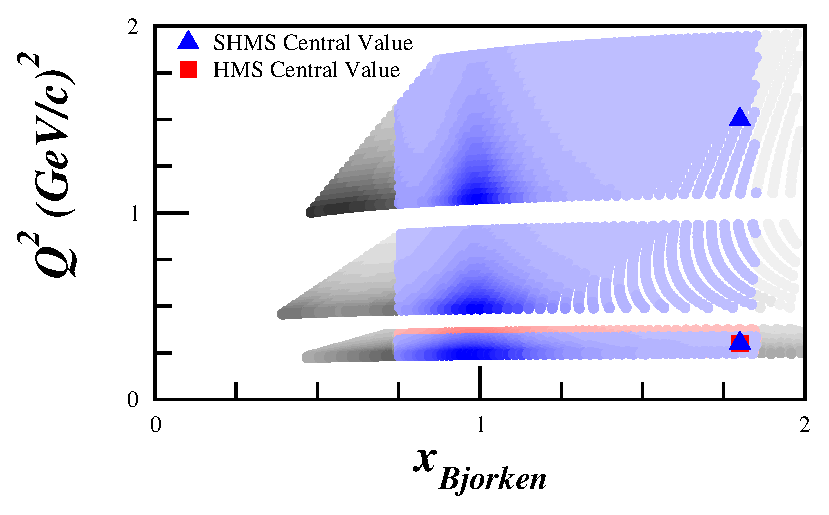
\includegraphics[width=0.49\textwidth]{figs/Pzz_30_all_q2.eps}~~
%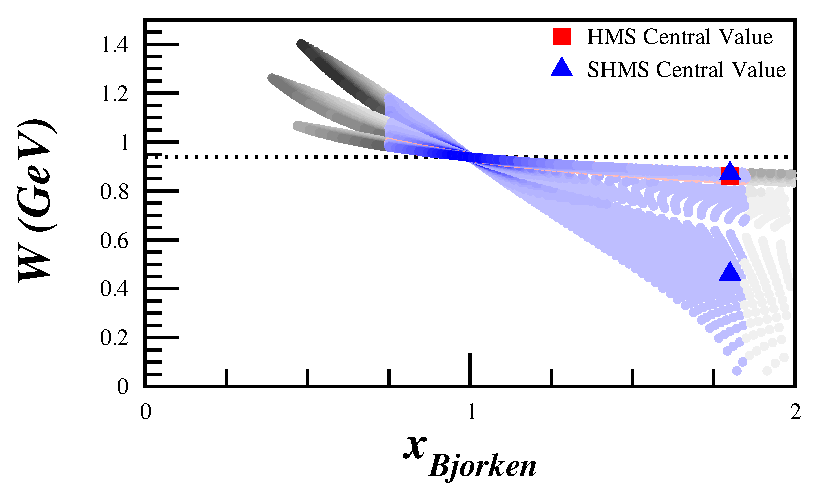
\includegraphics[width=0.49\textwidth]{figs/Pzz_30_all_w.eps} %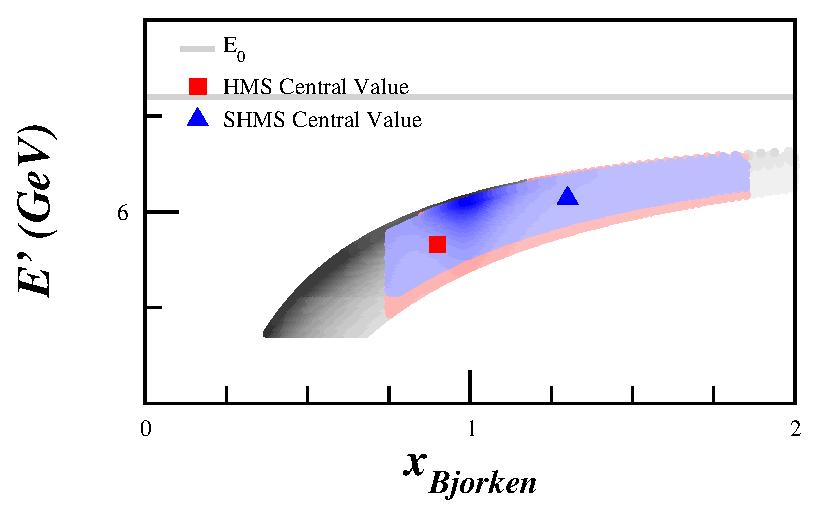
\includegraphics[width=0.49\textwidth]{figs/kine/Pzz_30_eprime.eps}
%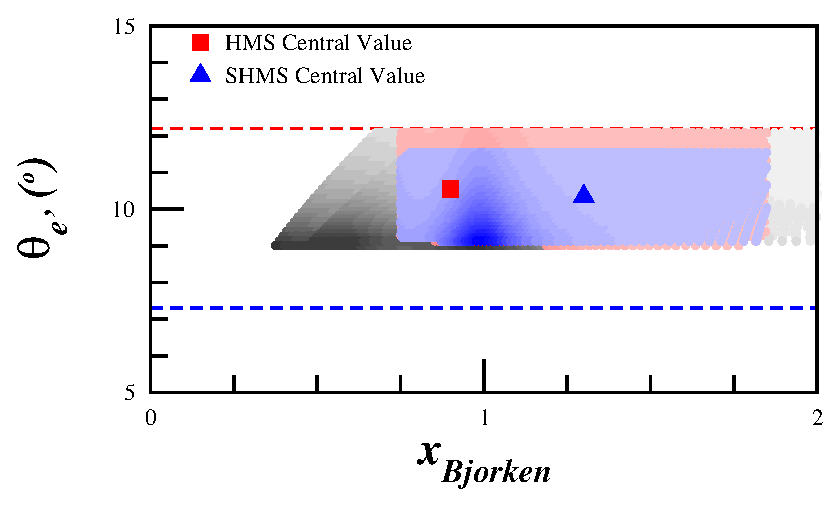
\includegraphics[width=0.49\textwidth]{figs/kine/Pzz_30_theta_eprime.eps}~~ 

\caption{\label{kincov} Kinematic coverage for central kinematic settings (not statistics weighted averaged) at $Q^2=1.5~(\mathrm{GeV}/c)^2$ (A), $0.7~(\mathrm{GeV}/c)^2$ (B), and $0.3~(\mathrm{GeV}/c)^2$ (C).  The grey regions are not included in our statistics estimates since they fall outside of $\XMIN < x < \XMAX$. Darker shading represents areas with higher statistics for each setting.}
\end{center}
\end{figure}


The polarized \TARGET target is discussed in section~\ref{POLTARGSEC}.  The magnetic field of the target will be held constant along the beamline at all times, while the target state is alternated between a polarized and unpolarized state.
The tensor polarization and packing fraction used in the rates estimate are \PZZ\% and \PF, respectively. 
The dilution fraction in the range of this measurement is shown in Fig.~\ref{fdil_plot}.
With an incident electron beam current of \CURRENT nA, the expected deuteron luminosity is \LUMI.
%$1.57\times 10^{35}$~cm$^{-2}}$s$^{-1}$.
%$?.??\times 10^{35}$~cm$^{-2}$s$^{-1}$.

The momentum bite and the acceptance were assumed to be $\Delta P = \pm 8\%$ and $\Delta\Omega = 5.6$~msr for the HMS, and $\Delta P= ^{+20\%}_{-8\%}$ 
%$-8<\Delta P <+20\%$
and $\Delta\Omega =4.4$~msr for the SHMS. 
%
For the choice of the kinematics,
special attention was taken onto the angular and momentum limits of the spectrometers: for the
HMS, $10.5^{\circ} \le \theta \le 85^{\circ}$ and $1 \le P_0 \le 7.3$ GeV/c, and for the SHMS,
$5.5^{\circ} \le \theta \le 40^{\circ}$ and $2 \le P_0 \le 11$ GeV/c. In addition, the
opening angle between the spectrometers is physically constrained to be larger than 17.5$^{\circ}$.
The dilution factors and projected uncertainties in $A_{zz}$ are summarized in Table~\ref{RATES2} and displayed in Fig.~\ref{PROJ}.  

\begin{figure}
\begin{center}
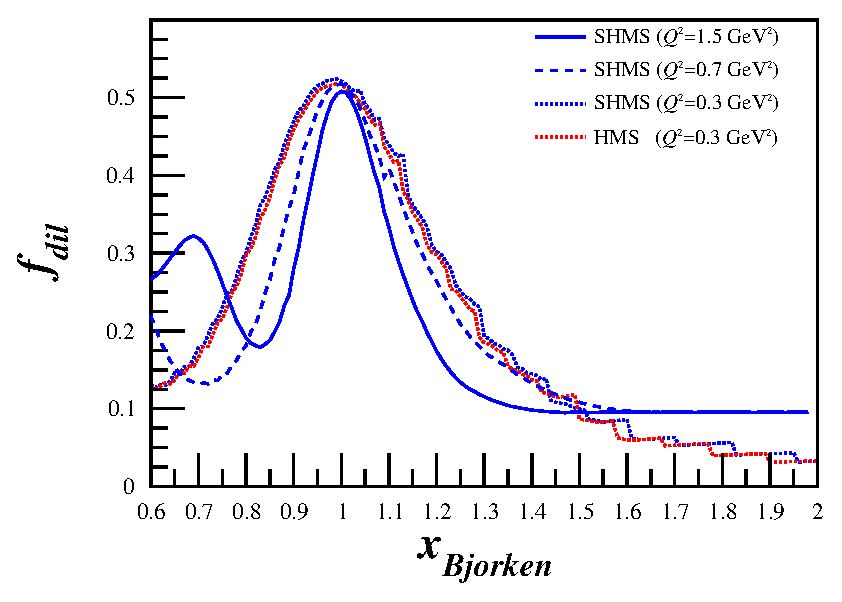
\includegraphics[width=0.5\textwidth]{figs/Pzz_30_fdil_all.eps} 
\caption{\label{fdil_plot}Projected dilution factor covering the entire $x$ range to be measured using a combination of P. Bosted's~\cite{Bosted:2012qc} and M. Sargsian's~\cite{misak-convo} code for the SHMS and HMS.}
\end{center}
\end{figure}

\begin{figure}
\begin{center}
%\includegraphics[width=0.45\textwidth]{figs/plots0705/b1_proj_newmiller_lin.eps}
%\hspace{0.5cm}
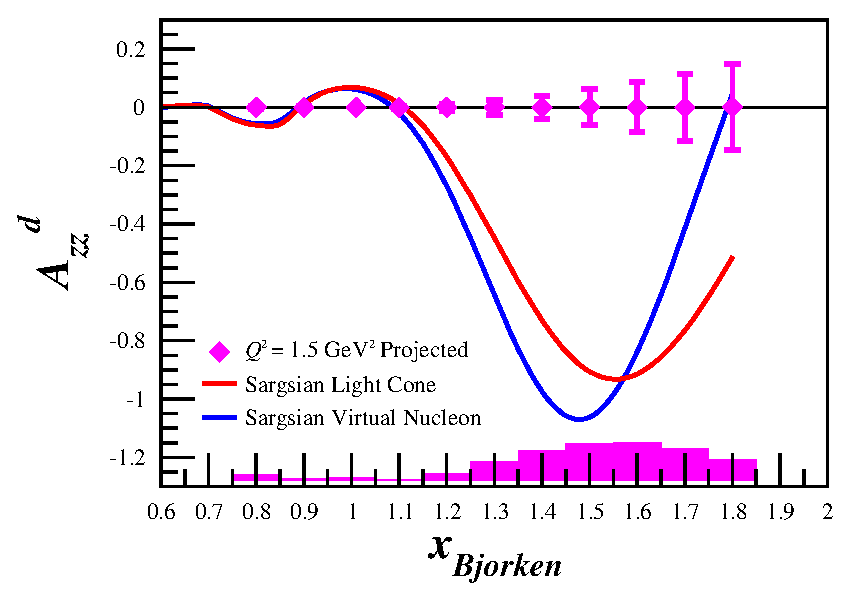
\includegraphics[width=0.75\textwidth]{figs/Pzz_30_q2_15_Azz_w_misak.eps} \\
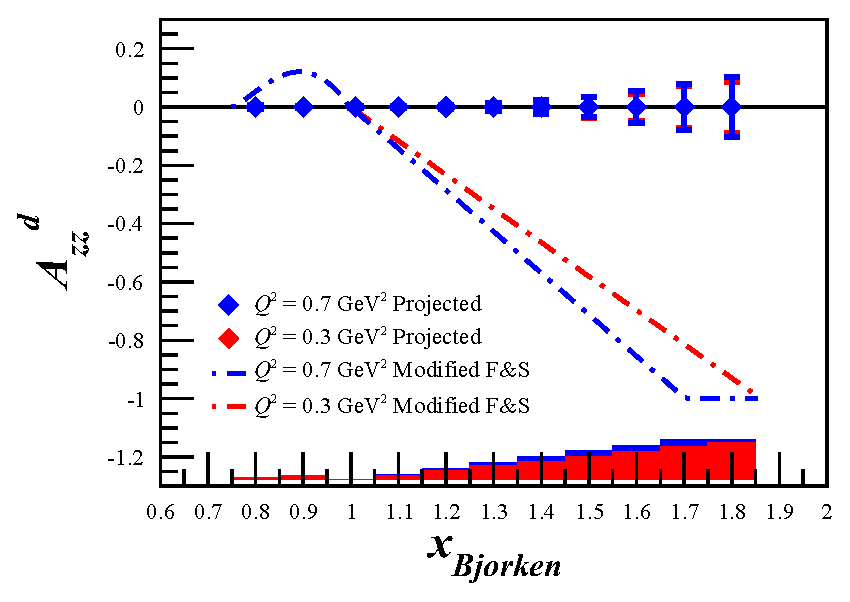
\includegraphics[width=0.75\textwidth]{figs/Pzz_30_q2_03_07_Azz_fs.eps} 
\caption{\label{PROJ}Projected statistical errors for the tensor asymmetry $A_{zz}$ with \productiondays days of beam time. The band represents the systematic uncertainty. Also shown for $Q^2=1.5~(\mathrm{GeV}/c)^2$ are calculations provided by M. Sargsian for using a light cone and virtual nucleon model, and for $Q^2=0.3$ and $0.7~(\mathrm{GeV}/c)^2$ a modified Frankfurt and Strikman model~\cite{Frankfurt:1988nt} that estimates the peak shifts in $x$ expected due to the SRC scaling changing with $Q^2$~\cite{Frankfurt:2008zv}.
}
\end{center}
\end{figure}

A total of \productiondays days of beam time is requested for production data, with an additional \overheaddays days of expected overhead.



\clearpage

%





